\begin{table*}
	\centering
	\renewcommand{\arraystretch}{1.25} \scriptsize
	\begin{tabular}{|*{14}{c|}}
		\hline
		\multirow{2}{*}{Users} & \multirow{2}{*}{Queued} & \multicolumn{3}{c|}{\multirow{2}{*}{Channel Gains}} & \multicolumn{3}{c|}{Q-WSRME approach} & \multicolumn{3}{c|}{\multirow{2}{*}{JSFRA Scheme}} & \multicolumn{3}{c|}{Q-WSRM band} \\
		\multirow{2}{*}{} & \multirow{2}{*}{Packets} & \multicolumn{3}{c|}{} & \multicolumn{3}{c|}{(modified \emph{backpreassure})} & \multicolumn{3}{c|}{} & \multicolumn{3}{c|}{Alloc Scheme} \\
		\cline{3-14}
		&& SC-\me{1} & SC-\me{2} & SC-\me{3} & SC-\me{1} & SC-\me{2} & SC-\me{3} & SC-\me{1} & SC-\me{2} & SC-\me{3} & SC-\me{1} & SC-\me{2} & SC-\me{3} \\
		\hline
		\me{1} & \me{4} & \me{1.71} &  \me{0.53}  &  \me{0.56} & \me{0} &  \me{0}  &  \me{0} & \me{4.0} &  \me{0}  &  \me{0} & \me{0} &  \me{0}  &  \me{0} \\
		\me{2} & \me{8} & \me{0.39} &  \me{1.41}  &  \me{1.03} & \me{0} &  \me{4.88}  &  \me{3.11} & \me{0} &  \me{5.49}  &  \me{0} & \me{0} &  \me{4.39}  &  \me{3.53} \\
		\me{3} & \me{4} & \me{2.34} &  \me{1.26}  &  \me{2.32} & \me{4.0} &  \me{0}  &  \me{0} & \me{0} &  \me{0}  &  \me{4.0} & \me{5.81} &  \me{0}  &  \me{0} \\
		\hline
		\multicolumn{5}{|c|}{Remaining backlogged packets (\me{\chi})} & \multicolumn{3}{c|}{\me{3.92} bits} & \multicolumn{3}{c|}{\me{2.51} bits} & \multicolumn{3}{c|}{\me{5.89} bits} \\
		\hline
	\end{tabular}
	\caption{Sub channel wise allocation for a scheduling instant}
	\label{tbl-1}
\end{table*}
%\begin{figure}
%\centering
%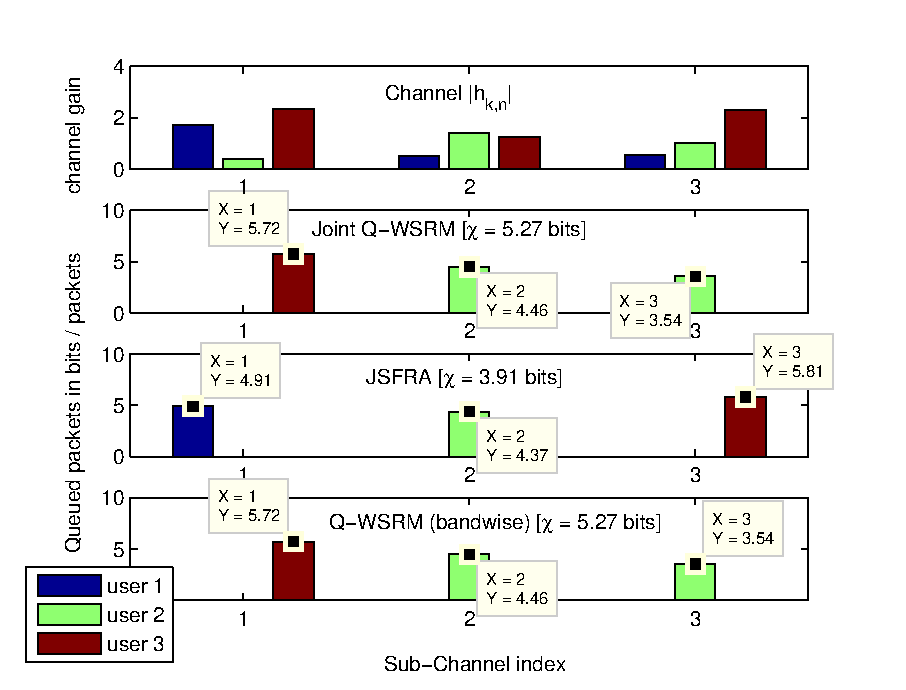
\includegraphics[width=\columnwidth]{tbl-1}
%\caption{Allocation for a \ac{SISO} Model comparing different Algorithms}
%\label{tbl-1}
%\end{figure}

In this section, we discuss the performance of the centralized algorithms from Section \ref{sec-3} for a few system configurations. To begin with, we consider a single cell \ac{SISO} model operating at \me{10} dB \ac{SNR} with \me{K = 3} users sharing \me{N = 3} sub-channel resources. The number of packets waiting at the transmitter for each user is given by \me{Q_k = 4,8} and \me{4} bits respectively. 

Table. \ref{tbl-1} outlines the channel seen by the users over each sub-channel followed by the rates assigned by three different algorithms, \ac{Q-WSRME} allocation, \ac{JSFRA} approach and the band-wise \ac{Q-WSRM} scheme using \ac{WMMSE} design \cite{wmmse_shi}. The performance metric used for the comparison is the total number of backlogged bits left over at each slot after the allocation, which is denoted by \me{\chi = \sum_{k = 1}^K \; [ Q_k - t_k ]^+}. Even though \me{\mc{U}(1)} and \me{\mc{U}(3)} has equal number of backlogged packets of \me{Q_{1} = Q_{3} = 4} bits, user \me{\mc{U}(3)} got scheduled in the first sub-channel due to the better channel condition. In contrast, the \ac{JSFRA} approach assigns the first user on the first sub-channel, which reduces the total number of backlogged packets waiting at the transmitter. The rate allocated for \me{\mc{U}(2)} on the second sub-channel is higher in \ac{JSFRA} scheme compared to the other schemes. It is due to the efficient allocation of the total power shared across the sub-channels.

For the \ac{MIMO} framework, we consider a system with \me{N=3} sub-channels and \me{N_B = 3} \acp{BS}, each equipped with \me{N_T = 4} transmit antennas operating at \me{10}dB \ac{SNR}, serving \me{|\mc{U}_b| = 3} users each. The path loss between the \acp{BS} and the users are uniformly generated from \me{[0,-3]} dB and the association is made by selecting the \ac{BS} with lowest path loss component. Fig. \ref{fig-1} shows the performance of the centralized schemes for a single receive antenna system. It compares the total number of \ac{SCA} updates required by the \ac{JSFRA}, \ac{SRA} and the \ac{Q-WSRME} schemes to perform the optimal allocations to minimize the total number of backlogged packets. The total number of queued packets for Fig. \ref{fig-1} is given by \me{Q_k = [14,15,14,8,12,9,12,11,11]} bits and for Fig. \ref{fig-2} is \me{Q_k = [9,12,8,12,5,4,10,8,5]} bits respectively.
\begin{figure*}
\centering
\subfloat[][System \me{\lbrace N,N_B,K,N_T,N_R \rbrace = \lbrace 4,3,9,4,1\rbrace}]{
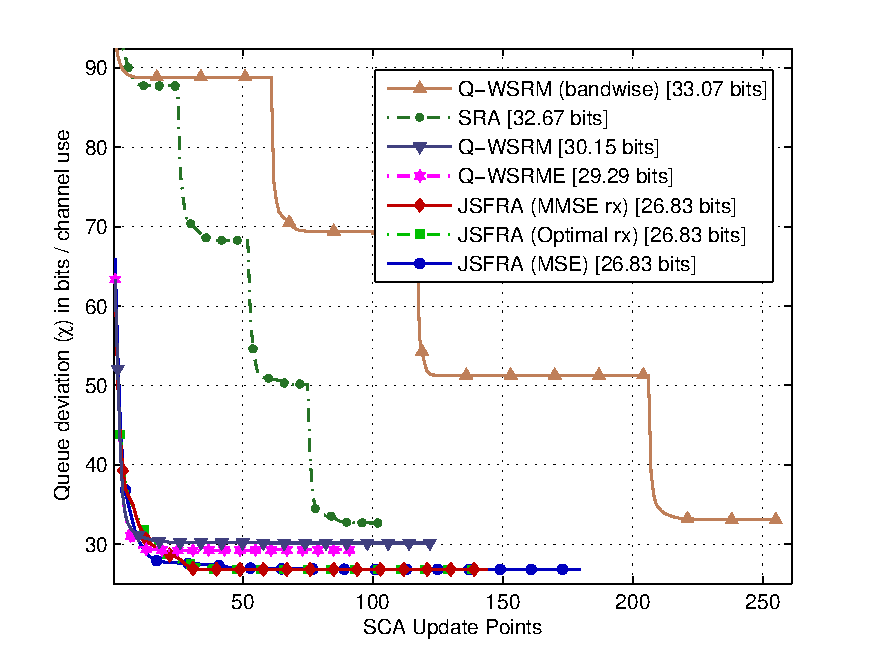
\includegraphics[width=0.48\textwidth]{fig-1-4}
\label{fig-1}}
\hfill
\subfloat[][System \me{\lbrace N,N_B,K,N_T,N_R \rbrace = \lbrace 2,3,9,4,2\rbrace}]{
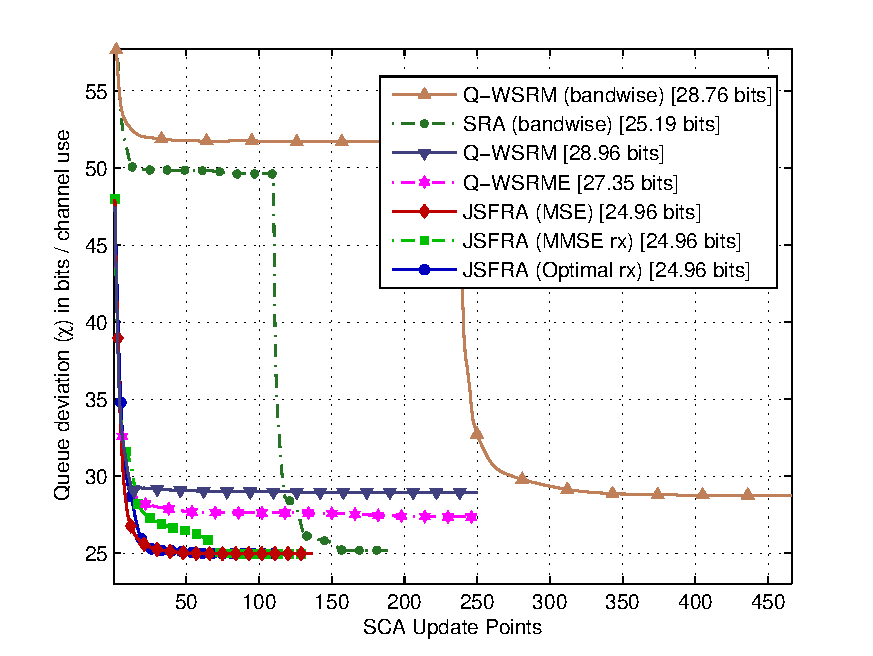
\includegraphics[width=0.48\textwidth]{fig-2-5}
\label{fig-2}}
\caption{Number of backlogged packets at the \ac{SCA} update points}
\label{fig-a}
\end{figure*}

The performance of the centralized algorithms are compared by the total number of residual bits remaining in the system after each \ac{SCA} update in Fig. \ref{fig-a}. The \ac{Q-WSRM} algorithm is not optimal due to the problem of over allocation when the number of queued packets are small, as in Fig. \ref{fig-a}. In contrast, the \ac{Q-WSRME} algorithm provides more favorable allocation by including the explicit rate constraint to avoid the over allocation problem. It can be seen that the \ac{JSFRA} algorithms converge to the optimal point for all formulations proposed in Section \ref{sec-3.2.1}. It can be seen that all the algorithms are Pareto-optimal and provides different performance based on the weights used to find a point in the rate region. 

In the scenario defined by Fig. \ref{fig-a}, \ac{Q-WSRME} performs marginally inferior to the \ac{JSFRA} algorithms due to the weights used in the rate maximization algorithm. The performance degradation can be attributed to the fact that the \ac{Q-WSRME} algorithm favors the users with the large number of backlogged packets as compared to the users with better channel conditions. Fig. \ref{fig-2} compares the algorithms for \me{N_R = 2} receive antenna case. In all figures, the receivers are updated along with the \ac{SCA} update instants \textit{i.e}, \me{J_{\max} = 1} in the Algorithm \ref{algo-1}. It is also noted that the performance degradation by performing the group update is very minimal. Since the receiver minimizes the objective for the fixed transmit precoders, the convergence is monotonic as can be seen from the figures.
\begin{table}
\flushleft
\renewcommand{\arraystretch}{1.25} \scriptsize
\begin{tabular}{|c|*{8}{c}|c|}
\hline
\me{q} & \multicolumn{8}{c|}{user indices} & \me{\chi} \\
\hline
\me{1} & 15.0 & 3.95 & 5.26 & 8.95 & 7.0 & 11.9 & 12.0 & 9.7 & 25.15 \\
\me{2} & 11.2 & 3.9 & 10.76 & 10.65 & 10.27 & 9.68 & 8.77 & 5.9 & 27.77 \\
\me{\infty} & 11.4 & 4.4 & 10.4 & 10.4 & 10.4 & 8.4 &  8.4 &  6.4 & 28.68 \\
\hline
\me{Q_k}  & 15.0 &  8.0 &  14.0 & 14.0 &  14.0 & 12.0 & 12.0 & 10.0  \\
\cline{1-9}
\end{tabular}
\caption{Queues for \me{\lbrace N,N_B,K,N_R \rbrace = \lbrace 5,2,8,1 \rbrace}}
\label{tbl-3} \vspace{-0.5cm}
\end{table}
%\begin{figure}
%\centering
%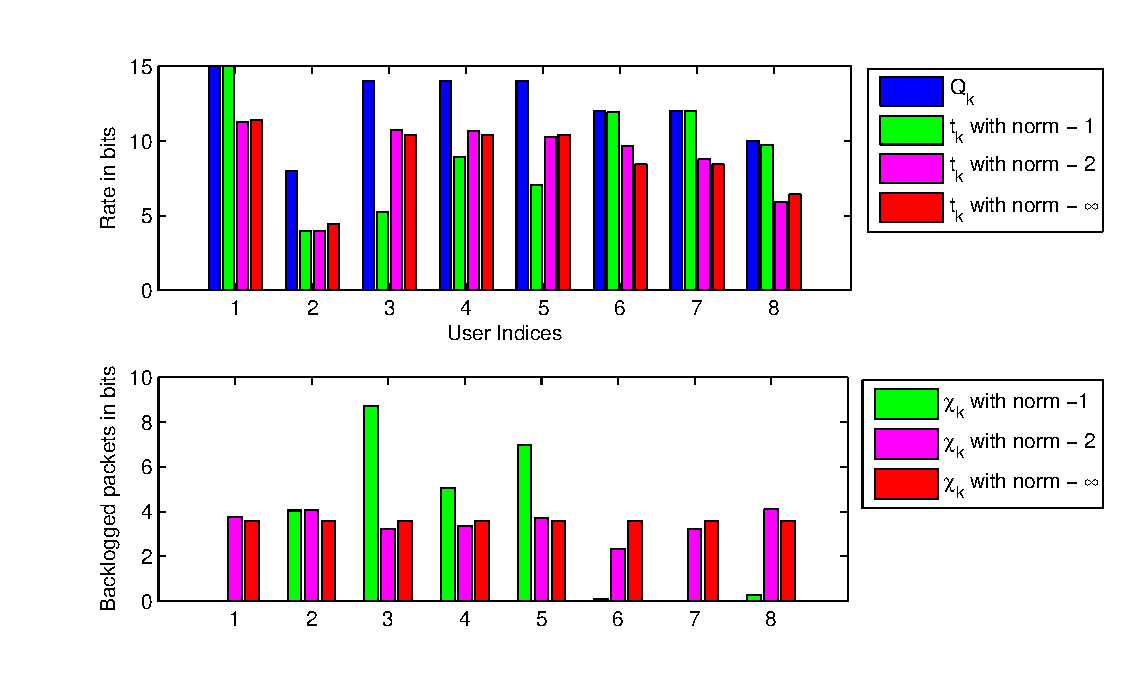
\includegraphics[width=\columnwidth]{tbl-2}
%\caption{Queue information for the system \me{\lbrace N,N_B,K,N_R \rbrace = \lbrace 5,2,8,1 \rbrace}}
%\label{tbl-3}
%\end{figure}

The behavior of the \ac{JSFRA} algorithm for different exponents \me{q} are outlined in the Table. \ref{tbl-3} for the users located at the cell-edge of the system employing \me{N_T = 4} transmit antennas. The configuration is mentioned in the caption of Table. \ref{tbl-3} along with the number of queued bits for each user. It is evident that the algorithm minimizes the queued bits for the \me{\ell_1} norm compared to the \me{\ell_2} norm, which is shown in the column displaying the total number of left over packets \me{\chi} in bits. The \me{\ell_{\infty}} norm provides fair allocation of the resources by making the left over packets to be equal for all users to \me{\chi_k = 3.58} bits. The \me{\ell_{\infty}} norm provides the fair allocation by making the queued deviation equal for all the users after the current allocation irrespective of their channel gains.
